\subsection{Gesteurte Gleichrichter}
\subsubsection{M1C}
\vspace{-0.5cm}
\begin{minipage}{0.4\linewidth}
    \includegraphics[width=\linewidth]{images/GRM1c}
\end{minipage}
\begin{minipage}{0.35\linewidth}
    \centering %BESSERE GRAFIK EINFèGEN
    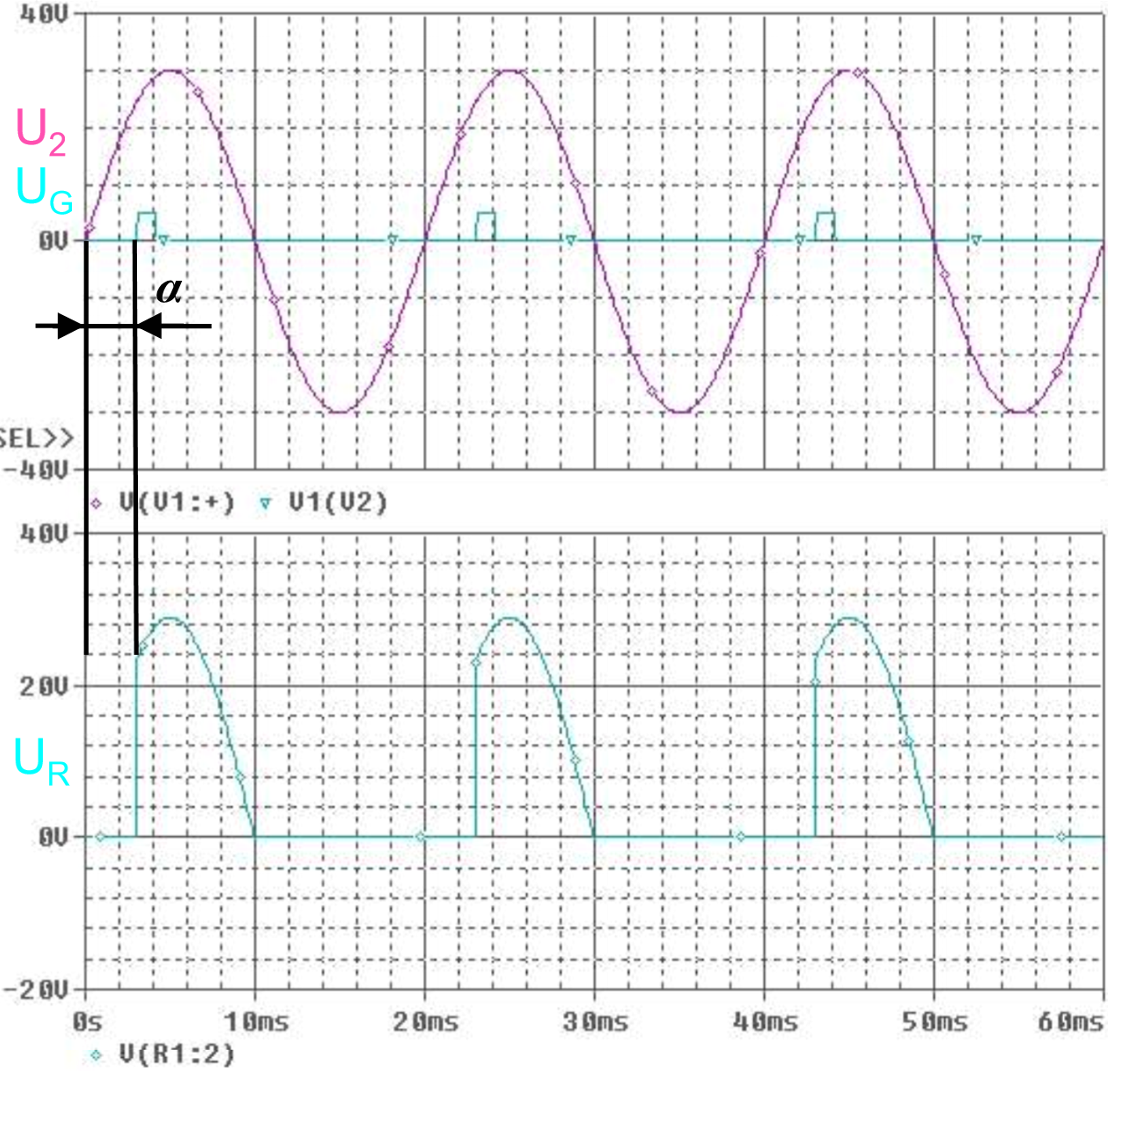
\includegraphics[width=\linewidth]{images/M1CKl}

\end{minipage}
\begin{minipage}{0.25\linewidth}
    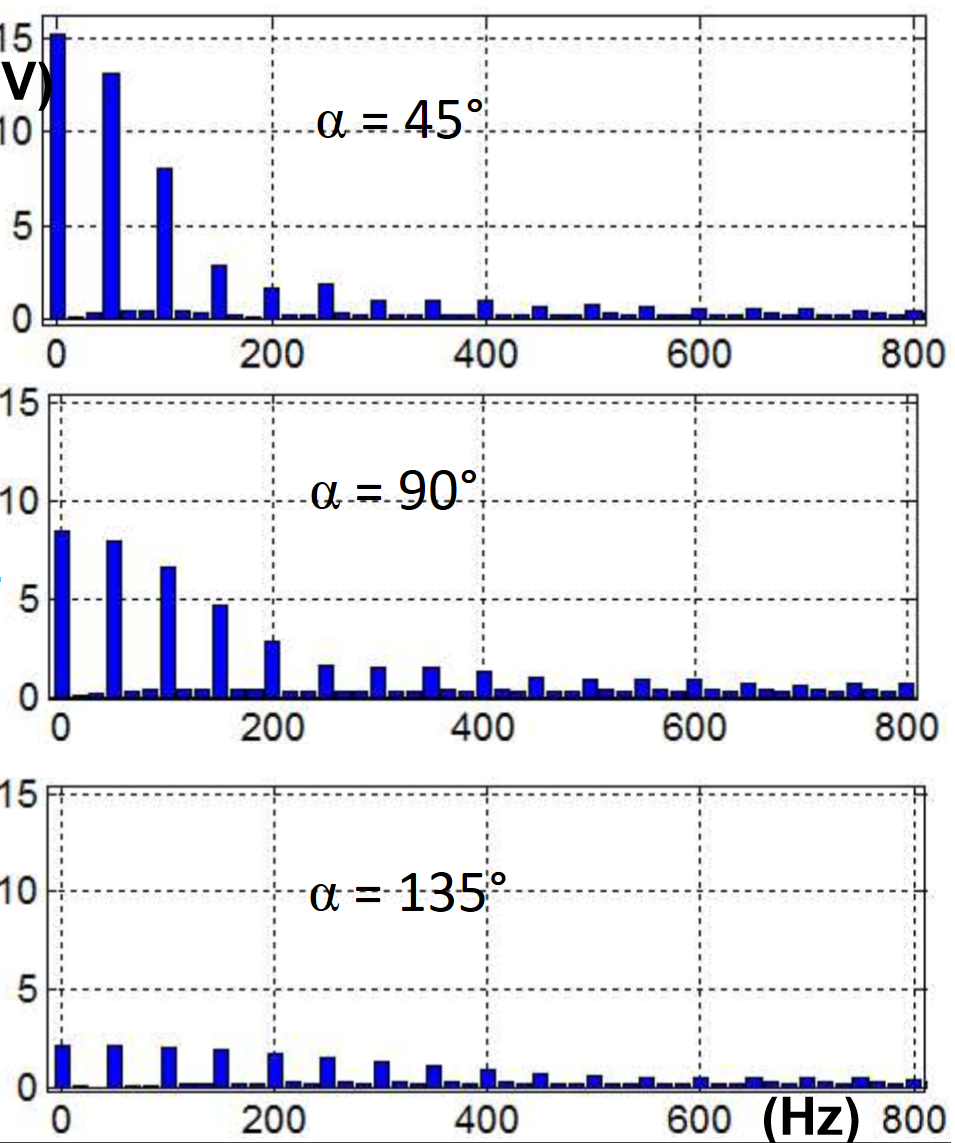
\includegraphics[width=\linewidth]{images/M1COW} 
\end{minipage}
\newline

\begin{longtable}{| p{.33\textwidth} | p{.40\textwidth} | p{.25\textwidth} |} %TODO Formeln einfügen
    \hline
    \textbf{Grundgleichungen}&
    \[ \bar{U}_{OUT} = \dfrac{1}{2\pi} \int\limits_{\alpha}^{\pi}\hat{U}_2\cdot sin(\beta) \diff \beta\]
    \[ \qquad \quad  =\dfrac{\hat{U}_2}{2\pi}(1+cos(\alpha)) \]&$ \beta = \omega t $\\
    \hline   
\end{longtable}


%===================================================================
%\clearpage

\subsubsection{B2C}

\begin{minipage}{0.4\linewidth}
    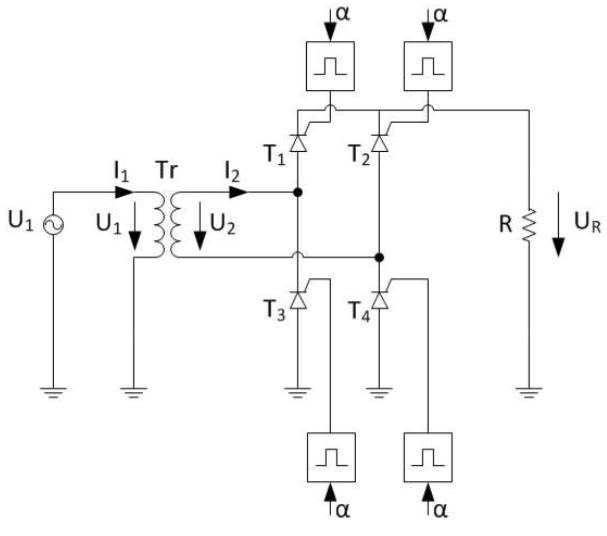
\includegraphics[width=0.8\linewidth]{images/GRB2c}
\end{minipage}
\begin{minipage}{0.35\linewidth}
    \centering 
    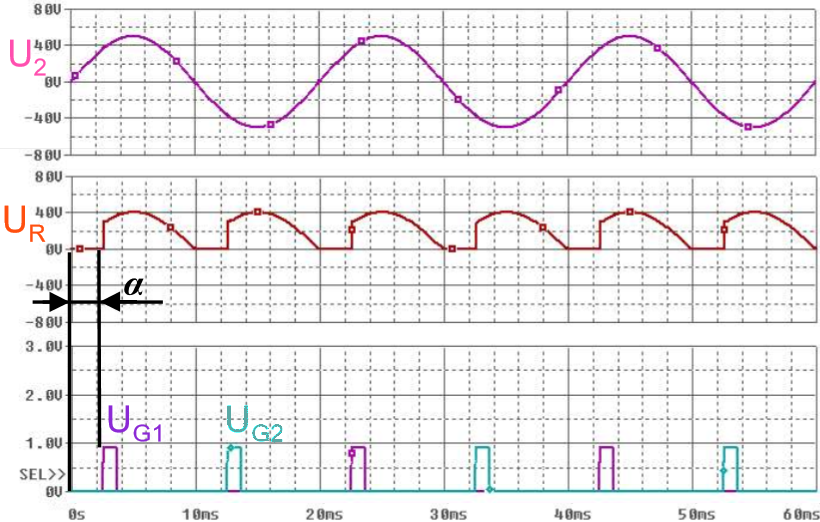
\includegraphics[width=\linewidth]{images/B2CKl}
    
\end{minipage}
\begin{minipage}{0.25\linewidth}
  todo Oberwellen grafik %TODO B2C \includegraphics[width=\linewidth]{images/B2COW} 
\end{minipage}
\newline

%===================================================================
%\clearpage


\subsubsection{B6C}%TODO B6C
\vspace{-0.5cm}
\begin{minipage}{0.4\linewidth}
    \includegraphics[width=\linewidth]{images/GRM1c}
\end{minipage}
\begin{minipage}{0.35\linewidth}
    \centering 
    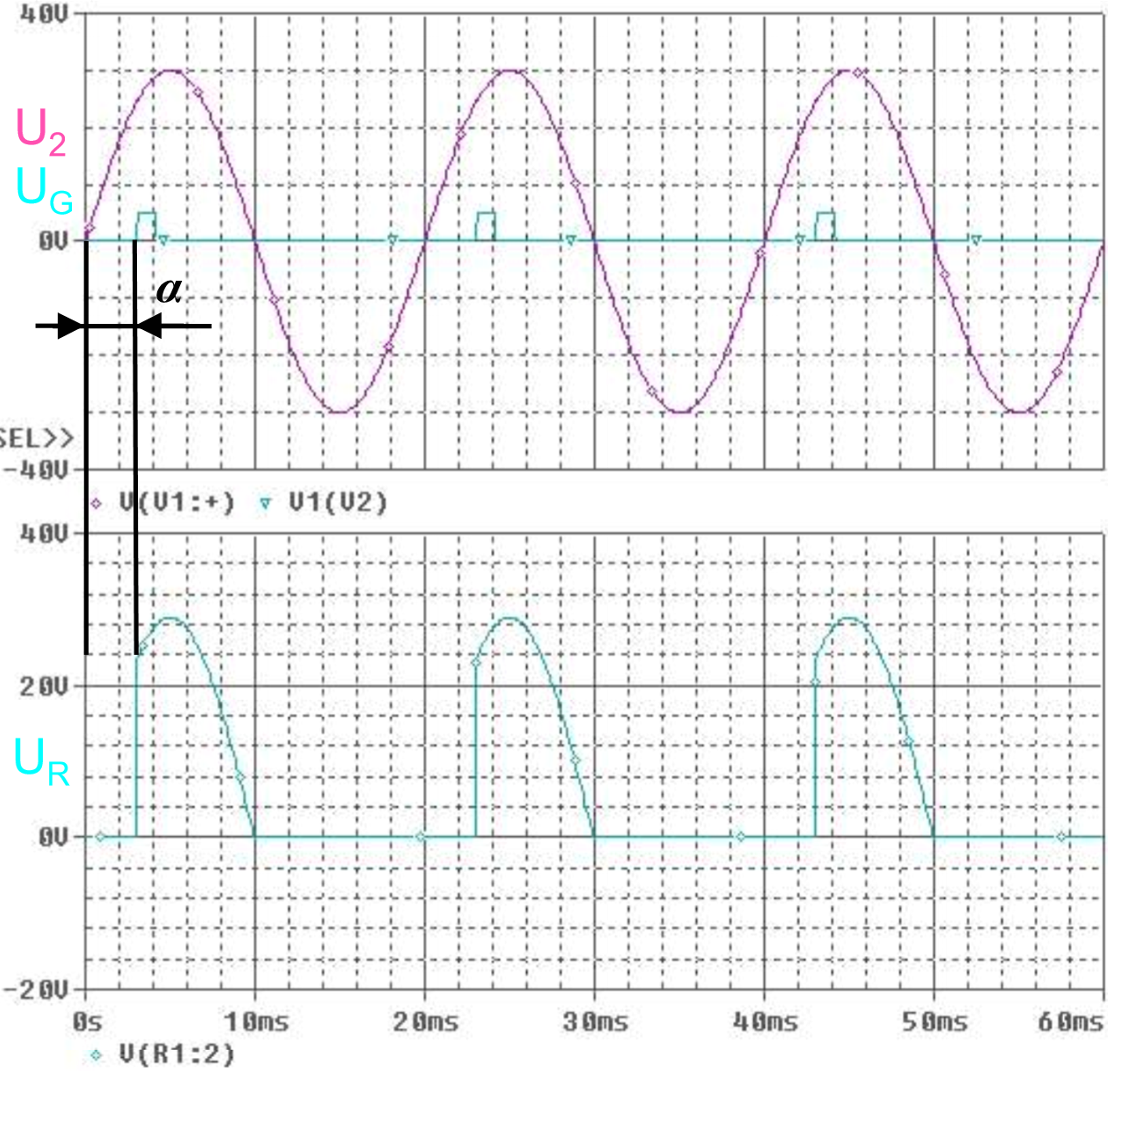
\includegraphics[width=\linewidth]{images/M1CKl}
    
\end{minipage}
\begin{minipage}{0.25\linewidth}
    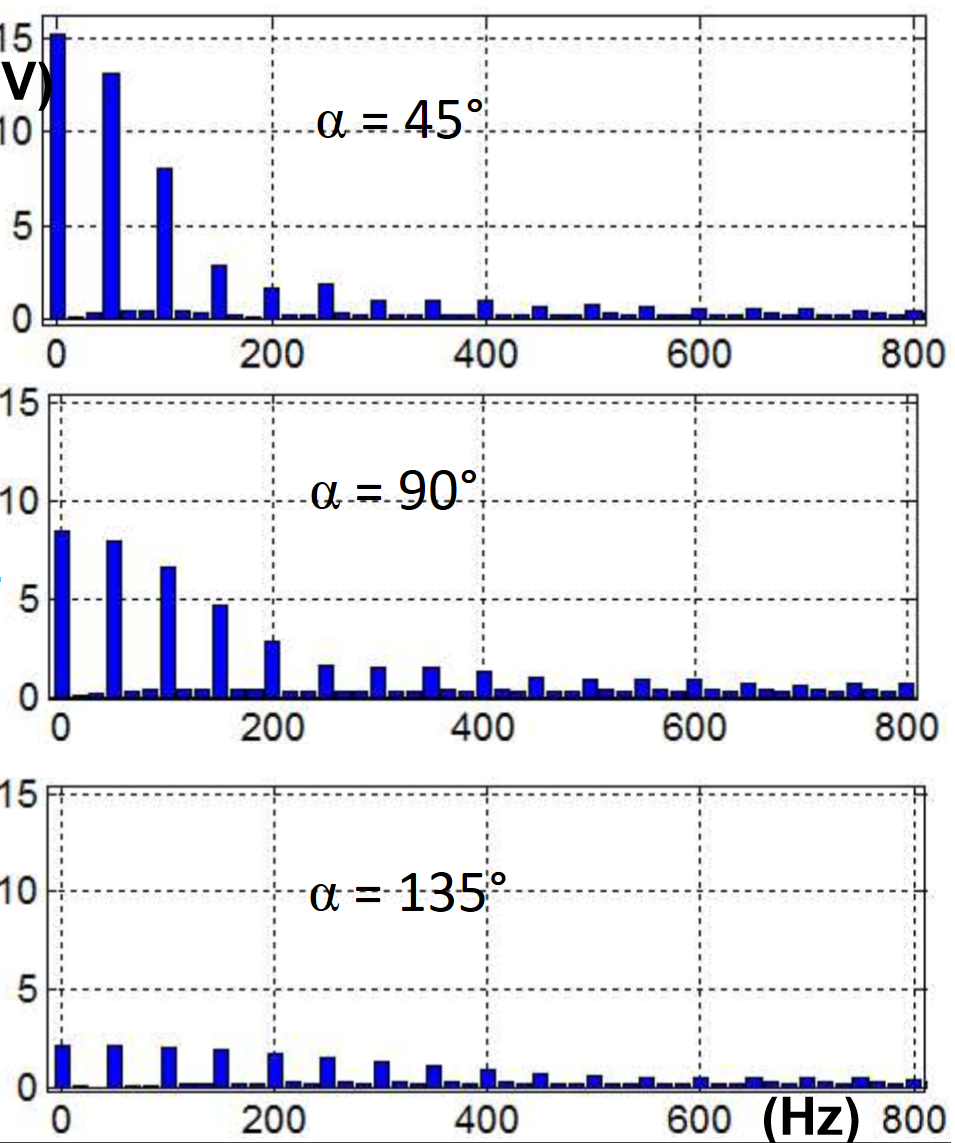
\includegraphics[width=\linewidth]{images/M1COW} 
\end{minipage}
\newline

%===================================================================
\clearpage